\subsection{Multimodal Learning} \label{sec:theory-approach-multimodal-learning}

\begin{figure}[t]
	\centering
	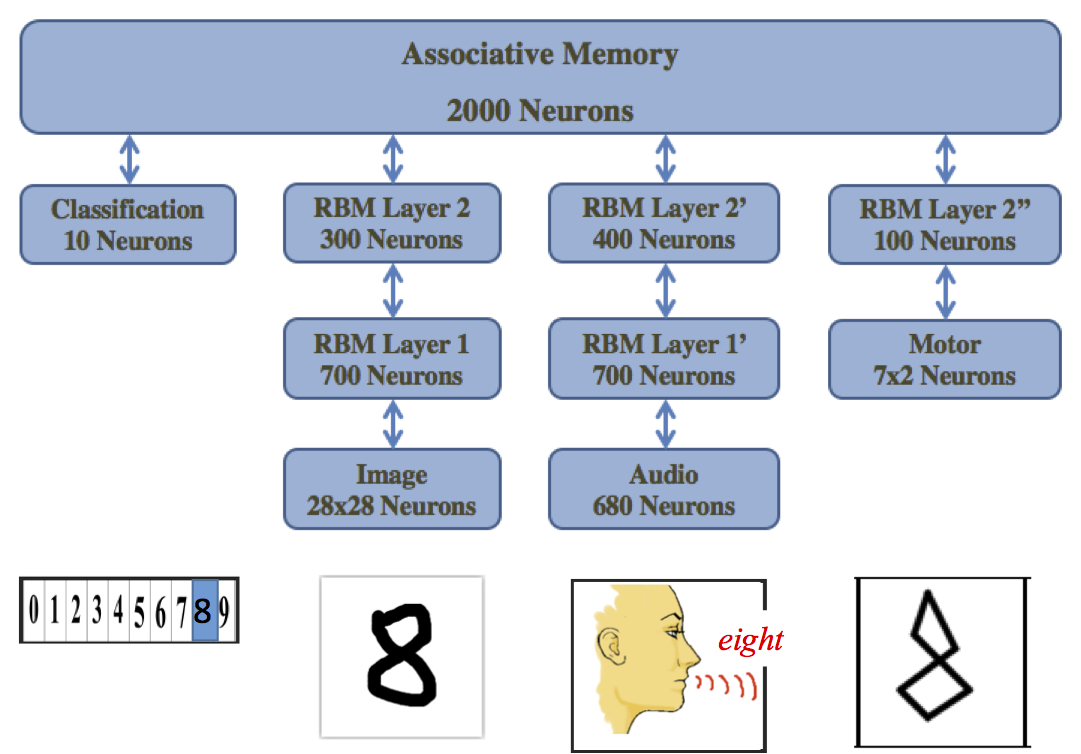
\includegraphics[max width=\textwidth]{multimodal-learning}
	\caption{A Multimodal neural network trained to communicate digits using several mediums. Each channel is modeled as a stack of Restricted Boltzman Machines connected to an associative layer\cite{iqbal2016scalable}.}
	\label{fig:multimodal-learning}
\end{figure}

Recent work by Iqbal and Silver (FLAIRS-2016 Best Paper Award)\cite{iqbal2016scalable} inspired by work by Hinton et al.\cite{Hinton:2006:FLA:1161603.1161605} and Srivastava et al.\cite{JMLR:v15:srivastava14b} has shown that it is possible to develop a multimodal deep learning system for learning a noisy handwritten digit using four sensor/motor channels (visual, audio, robotic, and symbolic) and an associative layer that ties all channels together.  After training, the presentation of a digit (sound, image, drawing) at the visible nodes of the model activates all other channels to create their associated reconstruction at their respective visible nodes. Each channel provides additional information that helps the other channels more accurately reconstruct the output. 

Figure \ref{fig:multimodal-learning} depicts the architecture that was developed as part of that work. Each channel is modeled as a stack of Restricted Boltzman Machines (RBM). A Restricted Boltzmann Machine is a generative neural network that can learn a probability distribution over its set of inputs. One important application of generative models is auto-encoding for feature engineering. Given a noisy input, an auto-encoder is able to extract a feature vector that is representative of the input based on the probability distribution being modeled\cite{pmlr-v5-salakhutdinov09a}.

\begin{figure}[t]
	\centering
	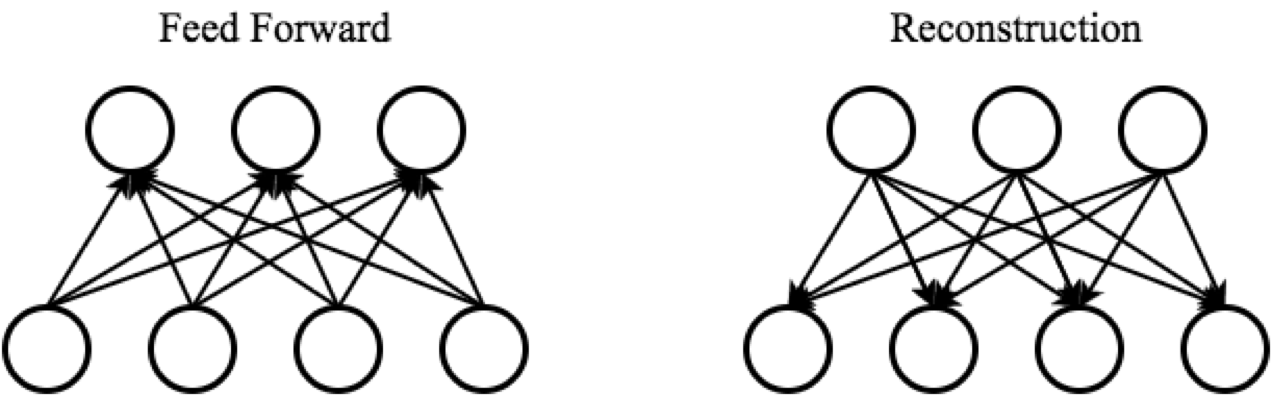
\includegraphics[max width=\textwidth]{rbm}
	\caption{An example of a Restricted Boltzman Machine showing the feed-forward pass and the reconstruction pass.}
	\label{fig:rbm}
\end{figure}

RBMs consist of an input layer and a hidden layer where the feature that represents the input is constructed. Training involves using the contrastive divergence (CD) algorithm to iteratively present the network with input examples, where an output is produced on the output layer during a feed-forward pass, and then the input is reconstructed back from that output. Figure \ref{fig:rbm} is a depiction of the architecture of an RBM showing the feed-forward and reconstruction passes. The goal of CD is to find an optimum set of weights that minimizes the reconstruction error. Contrastive divergence is an unsupervised process since there are no labels associated with the data. When fully trained, the output of RBMs is treated as a representation of the inputs that can be used in other machine learning tasks as is the case with deep belief networks\cite{Hinton:2006:FLA:1161603.1161605}.

The multimodal model developed by Iqbal and Silver\cite{iqbal2016scalable} learns to reconstruct the input presented to one channel on the other three channels each in their respective format (image, sound, robotic motion and symbol). The symbolic channel outputs the clearest signal as to which digit the multimodal deep learning system is ``thinking" about, given the input on the other channels. The symbolic channel also provides the clearest input for the other channels to generate the correct reconstructions at their visible nodes. This led us to a paper by Bengio\cite{DBLP:journals/corr/abs-1203-2990} that discusses the value of symbols and language in helping individuals learn concepts effectively without having to see all possible examples of that concept. This knowledge transfer in the form of symbols has a profound impact upon the development of our culture and the human species. 

Multimodal learning has inspired us to consider developing learning agents that learn to perform arithmetic operations using noisy channels but which can at times also receive concise information on a symbolic channel about the data on the noisy channels. The conjecture is that symbols are predominantly external communication tools that allow agents to share otherwise complex noisy concepts and in this way help them avoid local minima in model development. Clear symbols develop abstract representations that provide beneficial inductive bias during learning, therefore reducing the number of examples required to accurately learn a new concept.